% % % % % % % % % % % % % % % % % % % % % % % % % % % % % % % % % % % % % % % %
%
%	This is a Latex template for the group work report in the course ELEC-C5340 Applied Signal
%	processing.
%
%	11/2015
%	Jussi Nieminen
%
%
%
%
%	Document setup.
%
%	The necessary packages for writing a basic article are included in this section. If you need 
%	additional packages, declare them here. You will find the actual text body after the package 
%	declarations.	
%	
% % % % % % % % % % % % % % % % % % % % % % % % % % % % % % % % % % % % % % % %

\documentclass[11pt, a4paper, oneside]{article}
\usepackage[T1]{fontenc}

% Text alignment
\setlength{\parindent}{0cm}
\setlength{\parskip}{0.8em}
\setlength{\textheight}{24.8cm}
\setlength{\voffset}{-1.5cm}

% Unicode input encoding
\usepackage[utf8]{inputenc}

% Language. Change to finnish if you write in finnish (or use both)
%\usepackage[english]{babel}
\usepackage[finnish]{babel}

% Microtype makes the text really neat.
\usepackage{microtype}

% Graphics package
\usepackage[pdftex]{graphicx}
\usepackage[export]{adjustbox}

% Package enabling subfigures. This means that you can use figures
% with automatic "numbering" and referencing.
\usepackage{subfigure}

% Extended equation and symbol functionality
\usepackage{amsmath}
\usepackage{amssymb}
\usepackage{xfrac}

% New fonts based on Aalto
\usepackage{fouriernc}
\usepackage[scaled]{helvet}
\renewcommand*\ttdefault{txtt}
%\usepackage{inconsolata}
%\usepackage{tgheros}

% NatBib load. Check NatBib reference with Google if you want to know more
% about its options. In short, it is possible to modify almost everything
% about the citation style.
\usepackage[square, numbers]{natbib}

% Formatting for captions.
\usepackage[hang,bf]{caption}

% Simplistic code highlighting
\usepackage{listings}


% % % % % % % % % % % % % % % % % % % % % % % % % % % % % % % % % % % % % % % %
%
%	The document begins here. 
%
% 	Edit the necessary fields in the title page. The abstract and the section headings are already
%	written for you. Simply fill in your text, figures and equations.
%
% % % % % % % % % % % % % % % % % % % % % % % % % % % % % % % % % % % % % % % %

\begin{document}




% Title page

\begin{titlepage}
	\begin{flushleft}
	
	% Change the Aalto logo according to your language (Finnish / English)
	
\includegraphics[trim=1.5cm 1.3cm 0 1.5cm,width=0.55\linewidth]{Aalto_ELEC_FI_13_RGB_1.png} \\
	%
\includegraphics[trim=1.5cm 1.3cm 0 1.5cm,width=0.55\linewidth]{Aalto_ELEC_EN_13_RGB_3.png} \\
ELEC-C5340 \\
Sovellettu digitaalinen signaalinkäsittely \\
	\end{flushleft}

%	\begin{tabular*}{\textwidth}{@{\extracolsep{\fill} } lr}
%	
\includegraphics[trim=1.5cm 1.3cm 0 1.5cm,width=0.55\linewidth]{Aalto_ELEC_FI_13_RGB_1.png}% & \today
%	\end{tabular*}

	\begin{center}
	\vskip 8.0cm

	% Insert your title here
	{\huge \bf Realtime Guitaramplifier model\par}
	\vskip 2.0em
	{\large \lineskip .5em
	\begin{tabular}[t]{lr} 

	% Put your names and student numbers here. The '&' inserts a tab between the two fields
	Roope Kiiski & 217974 \\
	Niko Lindvall & number \\
	Alvar Wegelius & 296623 \\
 	\end{tabular} \par}

	\end{center}
	\vfill
	% Date is filled in automatically to the bottom of the page by using \today
	{\large \today\par}

\end{titlepage}




% First page

\begin{center}

	% Insert your title here
	{\LARGE \bf  Reaaliaikainen kitaravahvistinmalli\par}
	\vskip 1.5em
	{\large \lineskip .5em

	% Put your names here. The two backslashes \\ inserts a newline
	Roope Kiiski  \\
	Niko Lindvall  \\
	Alvar Wegelius  \\
 	\vskip 2.0em \par}

\end{center}

% Abstract

\begin{abstract}
\emph{Työn tavoitteena oli ohjelmoida C++:lla Juce-ympäristöä käyttäen reaaliaikaisesti toimiva kitaravahvistinmalli VSD-pluginina. 
Työssä on mallinnettu kitaravahvistimen eri putkiasteet sekä ekvalisaattori. 
Lisäksi laskostumisen minimioimiseksi käytettiin mallissa up- ja down-samplaysta. 
Lisäksi kokeilimme toteuttaa kaiutinmallin, mutta sen totesimme toimimattomaksi.}
\end{abstract}




% Document text

\section{Johdanto}

Kitaravahvistin on laite, jota käytetään sähkökitaraa soittaessa luomaan soittimelle ja soittajalle ominainen ääni.
Historiallisesti putkivahvistimia on käytetty erittäin paljon, koska monet soittajat kokevat niiden äänen olevan mielyttävämpi ja monipuolisempi kuin transistorivahvistimien. 
Putkivahvistimet ovat kuitenkin painavia, herkkiä kolahduksille ja usein myös hyvin kalliita laitteita. 
Kuitenkin koko ajan musiikkimaailma on siirtymässä kohti digitalisia versioita soittimistaan sekä vahvistimistaan, joten on tärkeää että myös kitaravahvistinmalleja luodaan, ja että ne kuulostavat hyvältä.
Digitaaliset kitaravahvistinmallit ovat merkittävästi halvempia, kestävämpiä sekä monipuolisempia kuin perinteiset vahvistimet, joten jos niistä saadaan riittävän hyviä, todennäköisesti ne yleistyvät nopeasti.
Tämän työn tarkoituksena on ohjelmoida kitaravahvistinmalli, joka kuulostaa oikealta, sekä jossa on kaikki kitaravahvistimen toiminnan kannalta tärkeät osat. 

\section{Metodit}

\subsection{Teoria ja algoritmit}

Kitaravahvistimen pääasiallinen tarkoitus on vahvistaa sähkökitarasta tuleva sähköinen signaali, mutta myös muokata sitä erilaisin tavoin, kuten esimerkiksi lisäämällä säröä. 
Yksi merkittävä ero kitaravahvistimen ja geneerisen vahvistimen välillä on se, että kitaravahvistimen taajuusvaste ei edes pyri olemaan lineaarinen. 
Säröä kitaravahvistin lisää joko leikkaamalla signaalia, tai vahvistamalla signaalia epälineaarisesti. . \cite{dafx}

Putkivahvistimet erityisesti tunnetaan omanlaisesta säröstään, joka johtuu vahvistinputkien siirtofunktion epälineaarisuudesta sekä siirtofunktion epäsymmetrisyydestä. 
Tämä on havainnollisetettu kuvassa \ref{fig:tube_transf}, jossa on esitetty ensimmäisen vahvistinasteemme putken siirtofunktio.. \cite{dafx}

\begin{figure}[h!]
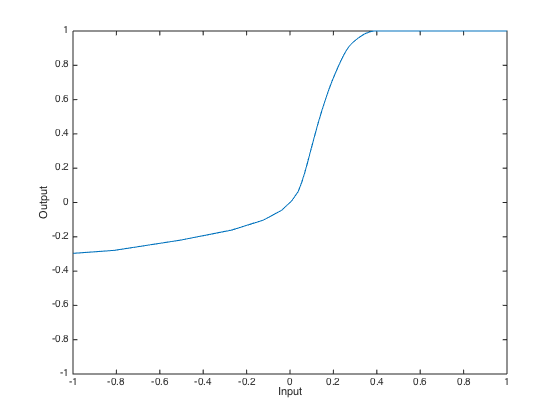
\includegraphics[width=1\textwidth, center]{tube_transf.png} \newline
\caption{Vahvistinputken siirtofunktio, josta nähdään ulostulevan ja sisäänmenevän signaalin suhde.}
\label{fig:tube_transf}
\end{figure}

Vahvistinputkessa särö syntyy, kun erivahvuuksiset sisääntulevat signaalit vahvistuvat eri verran, jolloin signaalin muoto vääristyy.
Erityisesti siirtofunktion epäsymmetrisyys, eli se, että positiiviset sisääntulon arvot vahvistuvat eri tavoin kuin vastaavat negatiiviset arvot, aiheuttaa sen, että vahvistinputken särö kuulostaa erilaiselta kuin transistorivahvistimen. 
Transistoreiden siirtofunktio on usein symmetrinen, ja sen seurauksena niiden muodostama särö on vain parittomia harmonisia, kun taas putken muodostama epäsymmetrinen särö sisältää myös parillisia harmonisia komponentteja. \cite{dafx}

Tässä työssä vahvistinputkea simuloidaan käyttämällä valmiiksi mitattujen vahvistinputkien siirtofunktiota. 

\subsection{Työkalut}

Kitaravahvistinmalli toteutettiin C++-kielellä käyttäen Juce-ympäristöä.
Käytännössä eri algoritmeja testattiin Matlabissa, ja kun ne todettiin toimiviksi, siirrettiin ne C++-koodiksi.  



\section{Toteutus}
 
 \subsection{Up- ja downsamplays}
 
 Upsamplayksessä saatujen näytteiden väliin lisätään nollia. Tämän jälkeen saatu output suodatetaan interpoloivan alipäästösuodattimen läpi.

Downsamplayksessä saatu input ensin alipäästösuodatetaan ja tämän jälkeen outputista poimitaan joka toinen arvo.

Up- ja downsamplayksessä käyettävät FIR-suodattimet osoittuivat ongelmallisiksi soittaessa aiheuttaen pauketta ja muita ongelmia. Korjausyrityksistä huolimatta suodattimet eivät toimineet halutulla tavalla joten pääätimme ottaa ne pois käytöstä. 


%Jos haluaa kirjoittaa koodia raporttiin, niin alla olevaa kannattaa hyödyntää:
%\begin{lstlisting}[frame=lines]{C}
%for n = 0:bufferLength
%	1. Calculate the nth output sample

%	2. Insert the input sample to the circular buffer
	
%	3. Increment the read and write pointer
%end
%\end{lstlisting}

 \subsection{Vahvistinasteet}
 
 Kitaramallimme toimii kolmella vahvistinasteella, joista toinen ja kolmas ovat putkimalliltaan identtiset, ja ensimmäinen erilainen, mutta muilta parametreiltaan kaikki kolme mallia ovat erilaisia.
 Tarkoituksena on simuloida vahvistimissa esiintyviä eri vahvistinasteita ja näin saada aikaan realistisempi ääni.
 Kuvassa \ref{fig:drive} on esitetty yksittäisen vahvistinasteen lohkokaavio. 
 
\begin{figure}[h!]
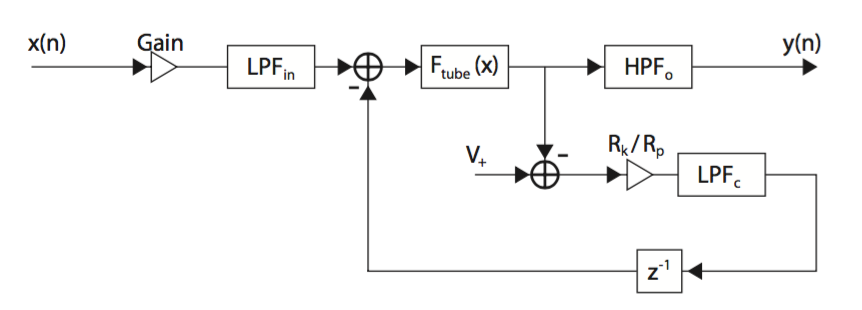
\includegraphics[width=1\textwidth, center]{drive.png} \newline
\caption{Vahvistinasteen lohkokaavio.}
\label{fig:drive}
\end{figure}

Lohkokaaviossa LPF-lohkot ovat alipäästösuodattimia, $F_tube$-lohko on putkimalli, sekä HPF-lohko on ylipäästösuodatin. 
 
 \subsection{Ekvalisaattori}

Ekvalisaattori päätettiin tähän työhön toteuttaa hydyntäen Fenderin '59 Bassmanin digitalisointia. 
Tarkoituksena on tällöin saada mahdollisimman aidon kuuloinen vahvistin, sekä todellista vastaava ekvalisaattorin toiminta. 
Kitaravahvistimien ekvalisaattorit eivät kuitenkaan koskaan ole ideaalisia, joten käyttämällä alipäästö-, kaistanpäästö, sekä ylipäästösuodattimia ekvalisaattorina, olisi lopputulos ollut kehno. \cite{fender}

Käytännössä Fenderin ekvalisaattori on toteutettu kuvassa \ref{fig:eq} esitetyn mukaisesti, ja se voidaan erilaisin matemaattisin operaatioin muuttaa muotoon joka on esitetty kaavassa \ref{eq:eq}. 
Kaavan kertoimet ovat tarkemmin avattu alkuperäisessä julkaisussa. \cite{fender}

\begin{figure}[h!]
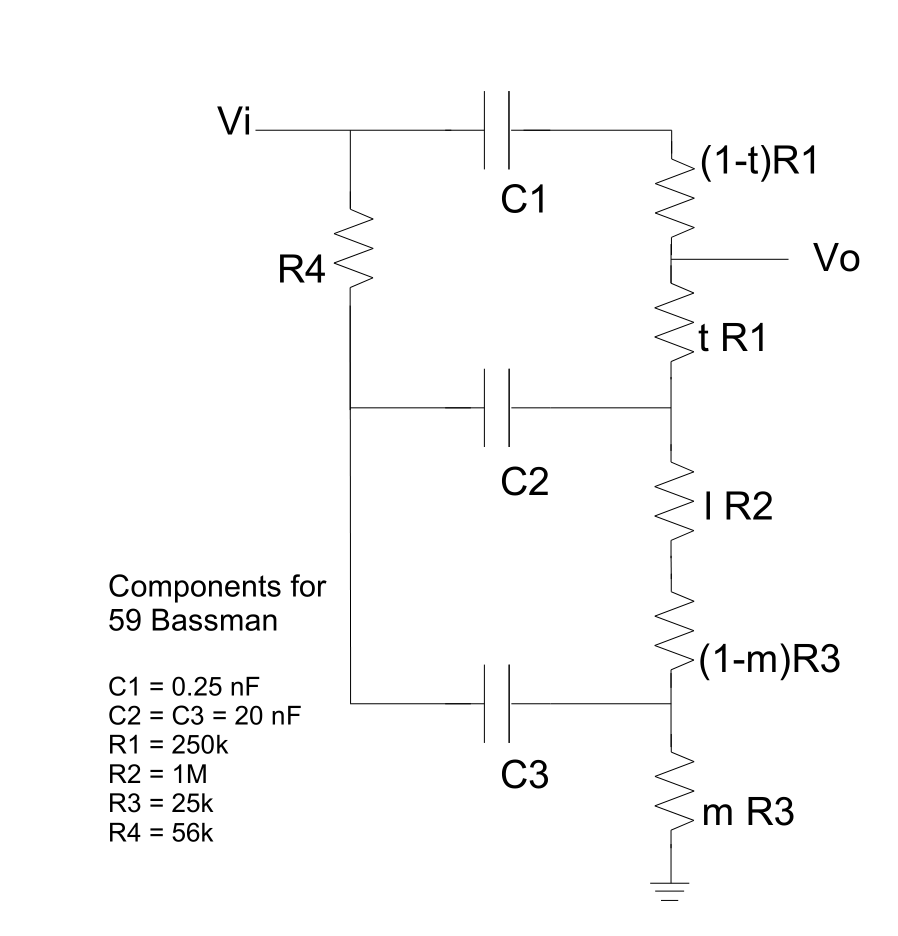
\includegraphics[width=0.8\textwidth, center]{eq.png} \newline
\caption{Fenderin '59 Bassman ekvalisaattorin kytkentä. \cite{fender}}
\label{fig:eq}
\end{figure}

\begin{equation}
H(z)=\frac{B_0 + B_1 z^{-1} + B_2 z^{-2} + B_3 z^{-3} }{A_0 + A_1 z^{-1}  + A_2 z^{-2}  + A_3 z^{-3} }
\label{eq:eq} % Kaavalle annetaan nimi
\end{equation} 

Käytännössä siis ekvalisaattori toteutetaan kolmannen asteen IIR-suodattimena, jonka kertoimet muuttuvat aina kun käyttäjä muuttaa ekvalisaattorin asetuksia. 
Tarkempi toiminta, kuten taajuusvasteet, on esitetty alkuperäisessä julkaisussa. \cite{fender}

 \subsection{Kaiutinmalli}
 
 Kaiutinmalli on myös erittäin keskeinen osa kitaravahvistimen ääntä, mutta meidän työssämme jouduimme jättämään sen pois, koska emme saaneet sitä toimimaan järkevästi. 
 Käytännössä kaiutinmalli on erittäin pitkä suodatin, ja suodattimen pituus aiheutti lukuisia ongelmia kuten pauketta, jota emme saaneet korjattua järkevällä työmäärällä.
 
\section{Tulokset}

Lopputulokseltaan kitaravahvistinmallimme toimii varsin hyvin. Särö kuulostaa varsin hyvältä, ekvalisaattori toimii kuten sen kuuluukin ja malli on reaaliaikainen. 
Kuitenkin ääni jättää paljon toivomisen varaan, sillä siinä on havaittavissa paljon erilaisia artefakteja, joita siinä ei pitäisi olla. 
Etenkin kun äänikortin bufferi asetetaan pieneksi, kasvaa ylimääräiset särökomponentit sekä naksunnat merkittävästi. 
Lisäksi myös jotkin filtterimme aiheuttavat ääneen havaittavaa ylimääräistä säröä.
Nämä ongelmat kuitenkin vaikuttavat olevan sellaisia, että niiden korjaaminen vaatii hyvin paljon perehtymistä ja aikaa, eikä se siten ole tämän kurssin puitteissa järkevää.


\section{Johtopäätökset}

Kokonaisuutena työ onnistui hyvin. 
Aikataulujen kanssa oli välillä haasteita, mutta kokonaisuudessaan saimme mallimme toimimaan kuten alunperin oli tarkoituskin, vaikka ääneen jäi lopulta parantamisen varaa.
Työstä mielenkiintoisen teki myös se, että eri ryhmän jäsenille eri asiat olivat uutta: osalle esimerkiksi C++-ohjelmointi oli uutta, kuten myös osalle Gitin käyttö versionhallinnointiin. 
Toisaalta myös itse reaaliaikaisuus toi ohjelmointiin uusia asioita.

Käytännössä tulevaisuudessa, jos työtä jatkaisi, pitäisi eri suodattimia parantaa, jotta eri artefaktit saadaan minimoitua.
Myös graaffista käyttöliittymää voisi hioa, siitä voisi ajan kanssa tehdä vaikka kuinka hienon, mutta tämän kurssin puitteissa siihen ei ollut järkevää käyttää liikaa aikaa.



\bibliographystyle{plain}
\bibliography{esim}

\end{document}
